\section*{Введение}
\addcontentsline{toc}{section}{Введение}
\label{sec:Introduction} \index{Introduction}
\large 

В наше время компьютерная обработка естественного языка является одной из самых
востребованных областей искусственного интеллекта. Для того, чтобы правильно
распознать смысл фразы, написанной человеком, необходимо иметь дополнительные
знания о каждом слове этого предложения и существующих связей между ними. К такой
вспомогательной информации относится отношение \textit{is-a}, что означает отношение
обобщения.

Способность к обобщению лежит в основе человеческого познания. Люди без труда могут
заменить частное на общее. Например, слово <<кошка>> на слово <<животное>>,
<<автомобиль>> на <<транспорт>>, <<красный>> на <<цвет>>. Для каждой пары общее слово имеет
термин \textit{гипероним}, а частное - \textit{гипоним}. Для каждого гипонима может существовать
несколько гиперонимов, и наоборот.


\begin{figure}[ht]
\centering 
    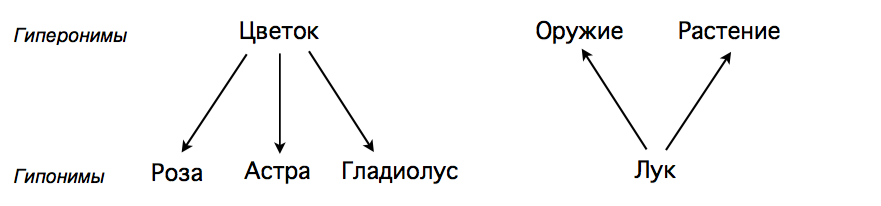
\includegraphics[scale=0.6]{image/Example.png}
    \caption{Пример связи гипонимов с гиперонимами.}
    \label{srg}
\end{figure}



Способность успешного распознавания таких лингвистических отношений приносит вклад
в такие области, как вопросно-ответная система, системы семантического поиска,
управление записями (система хранения и отслеживания документов), а также
информационный поиск и навигация по сайтам.

Например, наличие информации, что слова <<гепард>> и <<животное>> связаны отношением
\textit{is-a}, может помочь при ответе на вопрос <<какое самое быстрое животное?>>. А система
информационного поиска сможет подобрать соответствующие сайты, при получении
такого же запроса.

В добавок, отношение гипоним-гипероним - это основа почти любой семантической сети и
таксономии (иерархической системы отношений сущностей определенной области
знаний). Наличие таких построенных структур, помогает при реферировании текста, т.е.
извлечении из него основного содержания или заданной информации с целью
письменного изложения.

Таким образом, проблема определения отношений обобщения весьма актуальна как в
области лингвистики, так и в области искусственного интеллекта.

На данный момент большинство ресурсов, позволяющих определять отношение
обобщения, написаны вручную, что очень дорого в плане их создания и поддержки в
актуальном состоянии. Ручные словари зачастую имеют не достаточно большую область
покрытия. К тому же, в большинстве случаев, нет возможности выставления вероятности
наличия связи непрерывной случайной величиной от 0 до 1, а лишь только дискретная
степень допустимости существования отношения. Например, 0 - нет связи, 1- слабая, 2 -
средняя, 3 - сильная. Таким образом, нет возможности определить, какое из слов в
качестве гиперонима подходит больше, если есть несколько кандидатов имеющих
одинаковую степень. Для современных задач, появляется необходимость создания
автоматической системы поиска связи гипоним-гипероним.

Существует два основных вида постановки задачи. Первая, наиболее распространенная,
это сопоставление каждой паре слов 1 или 0, в зависимости от того, есть связь или нет.
Такого рода задача бинарной классификации неоднократно подвергалась критике за её
чрезмерную простоту, а также из-за невозможности сравнения кандидатов, как и в случае
ручных словарей. Второй способ заключается в поиске гиперонимов, т. е. предоставлении
ранжированного списка слов, которые наиболее вероятно являются гиперонимами
заранее заданному гипониму. Поиск таких слов происходит из конкретного словаря,
приближенному к словарю всех слов и устойчивых выражений для определенного языка.

В данной работе исследуется второй вид постановки задачи - поиск гиперонимов.
Рассматриваются различные алгоритмы, как с применением машинного обучения, так и
основанные на текстовых шаблонах. И производится сравнение полученных результатов
по различиям метрикам качества.





